Metal films were fabricated using a standard top-down plasma sputtering process
in Argon plasma at a pressure of \SI{1}{\milli\torr} and a gas flow rate of
\SI{12}{STP}.  The deposition rates were \SI{6.60}{\angstrom\per\second} for
gold and \SI{5.88}{\angstrom\per\second} for silver at 150 and \SI{66}{\watt}
DC, respectively.  During sputtering, the samples were rotated at \SI{50}{RPM}.
Though adhesion of the metal films to both glass and fluoropolymer substrates
was poor, instances of in-situ film-substrate separation were rare ($\sim5$
times over the course of hundreds of experiments).  Film-substrate separation
was observed to be instigated by stresses caused by pressure differentials in
the microfluidic flow cell.  The majority of such stresses were mitigated by
employing the siphon effect to flow liquids in the microfluidic cell in lieu of
mechanically forced flow.

%\begin{figure}
%\centering
%\includegraphics[keepaspectratio,width=5cm]{experimental/figures/SEM-nanoparticles.pdf}
%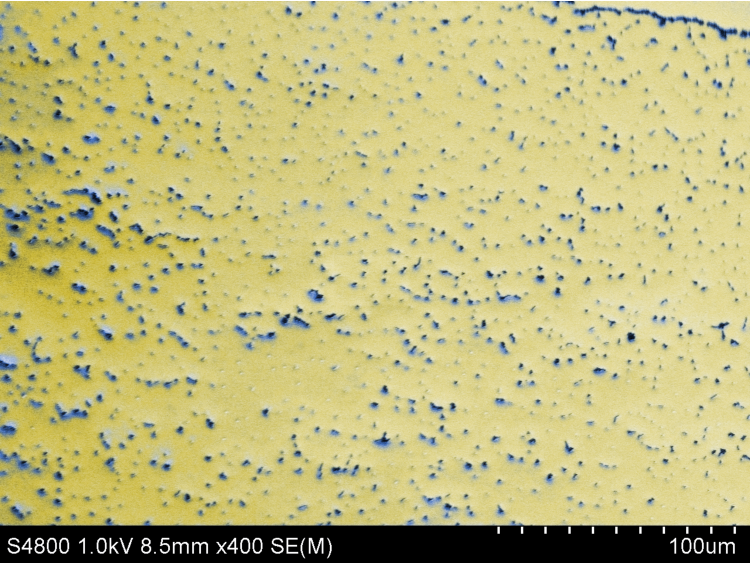
\includegraphics[keepaspectratio,width=5cm]{experimental/figures/SEM-holesa.pdf}
%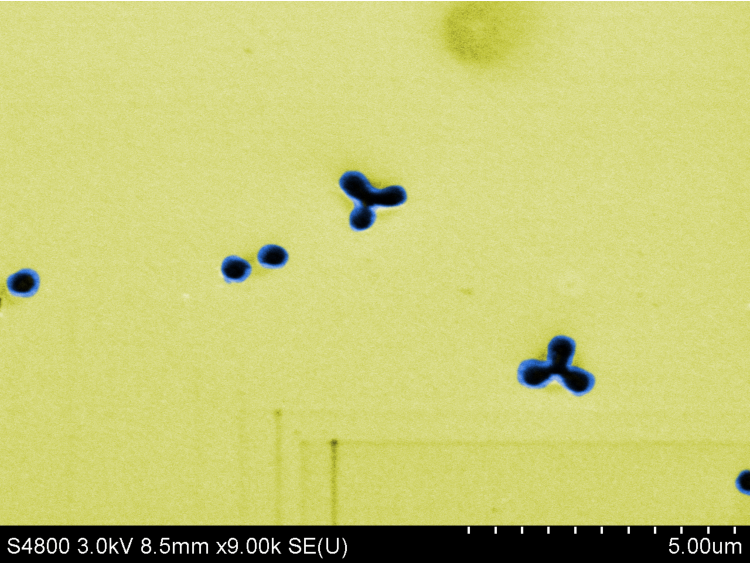
\includegraphics[keepaspectratio,width=5cm]{experimental/figures/SEM-holesb.pdf}
%\caption{SEM images of typical films produced with the plasma sputtering
%technique using the base set of parameters described in the text.}
%\label{fig:semsputter}
%\end{figure}

The substrate material consisted of a \SI{12}{\milli\meter} diameter BK7
N\raisebox{0.25em}{\relsize{-2}\b{o}}~1 glass coverslip.  Coverslips were
cleaned in a hot base bath.  A \SI{2}{\percent} solution of Hellmanex II was
first prepared in a pyrex beaker with a volume of \SI{25}{\milli\liter} and
heated to a temperature of \SI{60}{\celsius} on a hot plate.  The BK7
coverslips were immersed for \SI{300}{\second}.  The beaker was then removed
from the hot plate and put in a sonicator for \SI{300}{\second}.  After
sonication, the coverslips were removed from the solution and washed liberally
with distilled water and dried under a dry nitrogen stream.  Cleaned
coverslips were stored individually on top of a small
\SI{1}{\milli\meter\cubed} piece of PDMS plasma bonded to a microscope
coverslip, and prepared batches were kept in a dark box until use.  Coverslips
sputtered with metal films were stored in the same manner, but always used
within one or two days to forestall contamination or possible oxidation in the
case of silver films.

In the scattering experiments described in \Chapter{ch:speckle}
and~\ref{ch:scatteringmicro}, the substrate was bonded to a hemispherical prism
using NOA89 UV-cured optical adhesive.  NOA89 is well characterized for optical
applications with a high spectral transmission and a refractive index of
approximately 1.51 across the visible and near IR\@.  The prism material
consisted of either BK7 or NOA89 cast in a hemispherical mould made from BK7
prisms cast in PDMS\@.  Once the BK7 prism was removed from the PDMS, the void
was filled with NOA89 and cured under a \SI{15}{\watt} UV lamp at a distance of
\SI{5}{\centi\meter} for \SI{12}{\hour}.  To remove bubbles, the UV adhesive
was first centrifuged in an opaque microcentrifuge tube at \SI{15000}{RPM} for
\SI{30}{\minute}.  As the substrate construction is independent of the prism
material and both NOA89 and BK7 have nearly the same refractive index
(approximately 1.51 at \SI{660}{\nano\meter}), the two cases are not
distinguished except to note that the NOA89 prisms are easier to fabricate in
bulk.

For the interference experiments in \Chapter{ch:interference}, prisms of
either LAH79 or BK7 were used with the metal film sputtered directly onto the
prism's hypotenuse.  Such glass prisms were prepared by first removing any
existing metal film.  Silver films were removed by immersion in
\SI{70}{\percent} \ce{HNO3} for \SI{60}{\second}.  Gold films were removed
similarly by immersion in freshly prepared aqua regia, composed of a 1:3 ratio
of \ce{HNO3} to \ce{HCl}.  The glass prisms were sonicated in acetone to
remove any organic contaminants and rinsed in ultra-pure dry acetone.
Finally, the surface was cleaned with methanol and lens tissue using the drag
and drop method.
